\lecture{1}{02-06-2023}{Analysis}

\section{``x-'' und ``h-'' Methode}
\subsection{Unterricht}
Berechnung der Ableitung mithilfe der ``x-Methode''
Beispiel: $f(x)=x^{3}; x_{0}=-2$ 
\begin{equation}
\text{mit:} \lim_{h \rightarrow 0} \frac{f(x+h)-f(x)}{h}
\end{equation}

\begin{align*}
     f'(-2) & = \lim_{x\to-2}\frac{f(x)-f(-2)}{x-(-2)} \\
			& = \lim_{x\to-2}\frac{x^{3}-(-2)^3}{x+2} \\
			& = \lim_{x\to-2}(x^{2}-2x+4) \\
			& = -2^{2}-2\cdot -2+4\\
			& = 4
\end{align*}

\subsection{Hausaufgaben}
\subsubsection{Aufgabe 1, berechnen sie $f'(x_0)$}
(a)	$f(x)=x;x_{0}=3 \implies 1$\\
(b)	$f(x)=x^{2};x_{0}=3 \implies 6$\\
(c)	$f(x)=\sqrt{x};x_{0}=4 \implies r: x^{\frac{1}{2}}=\frac{1}{2}x^{-1/2}\implies ,25$\\
(d)	$f(x)=\frac{1}{x};x_{0}=-1 \implies x^{-1}=-1^{-2}=-1$

\subsubsection{Aufgabe 2, berechnen sie $f'(x_0)$}
(a)	$f(x)=x;x_{0}=1 \implies 1$\\
(b)	$f(x)=x^{2};x_{0}=-4 \implies -8$\\
(c)	$f(x)=\sqrt{x};x_{0}=4 \implies r: x^{\frac{1}{2}}=\frac{1}{2}x^{-1/2}\implies ,125$\\
(d)	$f(x)=\frac{1}{x};x_{0}=3 \implies x^{-1}=-1x^{-2}=-3^{-2}=-\frac{1}{9}$

\subsubsection{Aufgabe 3}
Für eine Bewegung mit konstanter Beschleunigung aus der Ruhe gilt für den
zurückgelegten Weg s (in m) in Abhängigkeit von Zeit t (in s) die Formel
\begin{equation*}
s(x)=\frac{1}{2}at^2.
\end{equation*}
Dabei ist a (in $\frac{m}{s^2}$) die Beschleunigung.\\
(a) Berechnen Sie den zurückgelegten Weg nach 3s bzw. 6s.\\
$s'(t)=at \implies$ 3a und 6a\\
(b) Die Momentangeschwindigkeit zum Zeitpunkt $t_0$ ist definiert als
\begin{equation*}
v(t_0)=s'(t_0)=\lim_{t \to t_0}\frac{s(t)-s(t_0)}{t-t_0}.
\end{equation*}

\clearpage
\section{Pascalsches Dreieck und Binomischer Lehrsatz, 16.1.2023}
\subsection{Unterricht}

\[f'(x_0)=\lim_{x \to x_0}\frac{f(x)-f(x_0)}{x-x_0}= \lim_{h \rightarrow 0} \frac{f(x+h)-f(x)}{h}\]
Beispiel: $f(x)=x^4; x_0 =3$
\[f'(5)= \lim_{h \to 0} \frac{f(x_0+h)-f(x_0)}{h} = \lim_{h \to 0}\frac{(5+h)^4-5^4}{h} \] \[= \lim_{h \to 0}\frac{5^4+4\cdot 5^3h+6\cdot 5^2\cdot h^2+4\cdot 5\cdot h^3+h^4-5^4}{h} \\ = \lim_{h \to 0}4\cdot 5^3+6\cdot 5^2\cdot h+4\cdot 5\cdot h^2+h^3=4\cdot 5^3=500\]\\


\begin{figure}[h]
\centering
\paragraph{Pascalsches Dreieck:}
\begin{tabular}{>{$n=}l<{$\hspace{12pt}}*{13}{c}}
0 &&&&&&&1&&&&&&\\
1 &&&&&&1&&1&&&&&\\
2 &&&&&1&&2&&1&&&&\\
3 &&&&1&&3&&3&&1&&&\\
4 &&&1&&4&&6&&4&&1&&\\
5 &&1&&5&&10&&10&&5&&1&\\
6 &1&&6&&15&&20&&15&&6&&1
\end{tabular}
\end{figure}

\textbf{Binomischer Lehrsatz:}
\[(x+y)^n = \sum_{k=0}^{n}\binom{n}{k} x^{n-k}y^{k} \quad\]
\begin{align*}
(x+y)^0 & = 1, \\[8pt]
(x+y)^1 & = x + y, \\[8pt]
(x+y)^2 & = x^2 + 2xy + y^2, \\[8pt]
(x+y)^3 & = x^3 + 3x^2y + 3xy^2 + y^3, \\[8pt]
(x+y)^4 & = x^4 + 4x^3y + 6x^2y^2 + 4xy^3 + y^4, \\[8pt]
(x+y)^5 & = x^5 + 5x^4y + 10x^3y^2 + 10x^2y^3 + 5xy^4 + y^5, \\[8pt]
(x+y)^6 & = x^6 + 6x^5y + 15x^4y^2 + 20x^3y^3 + 15x^2y^4 + 6xy^5 + y^6, \\[8pt]
(x+y)^7 & = x^7 + 7x^6y + 21x^5y^2 + 35x^4y^3 + 35x^3y^4 + 21x^2y^5 + 7xy^6 + y^7, \\[8pt]
(x+y)^8 & = x^8 + 8x^7y + 28x^6y^2 + 56x^5y^3 + 70x^4y^4 + 56x^3y^5 + 28x^2y^6 + 8xy^7 + y^8.
\end{align*}
\clearpage


\section{``h-Methode''}
\subsection{Unterricht}
Bis jetzt nur ``h-Methode'' gemacht. Deswegen hier private Aufgaben, dass es nicht leer ist.
\\\textbf{Chapter 2 Exercises - Part A, 4}
\[\frac{d}{dx}\left[\frac{3-2x^2}{4-3x^2}\right]= \frac{(4-3x^2)\left( \frac{d}{dx}\left[4-3y^2\right]
 \right)-(3-x^2)\frac{d}{dx}\left[4-3x^2\right]
}{\left( 4-3x^2 \right)^2 }\]\[= \frac{(4-3x^2)(-4x)-(3-2x^2)(-6x)}{16-12x^2-12x^2+9x^4}= \frac{2x}{16-24x^2+9x^4} \]
\textbf{Buch, Aufgabe 13}
\\a) Man kann hier zwar $\lim_{h \to 0^+ } $und $ \lim_{h \to 0^-}$, wo es von links -1 ergibt und rechts 1. Hier gibt es zwar links und rechts eine Tangente der Steigung, aber da die nicht gleich sind gibt es kein limit generell.
\[ \text{Wenn} \lim_{h \to 0^+ } \ne \lim_{h \to 0^-} \implies \lim_{h \to 0} \textbf{D.N.E.}\]
b) $x=3$



\clearpage
\section{Arbeit Verbesserung}
\subsection*{Taschenrechnerfrei}
\textbf{Aufgabe 1}
\[(u\circ v)(x)=e^{\frac{1}{2}\frac{1}{x^2+1}} ; (v\circ u)(x)=\frac{1}{e^x+1} \]
\textbf{Aufgabe 2.1}
Ist wahr, da:
\begin{align*}
    g(x) & =1-x  \to\\
        y &= 1-x\\
        y+x & = 1\\
        x & = 1-y\\
        f^1{-1}(x) & =1-x\\
\end{align*}
\textbf{Aufgabe 2.2}
Ist Wahr, da im Nenner immer in x mehr ist als im Zähler, dies verhindert das $y=1$ wird.

\noindent\textbf{Aufgabe 3}


\subsection*{Taschenrechner Teil}
\textbf{Aufgabe 1.1}
Hier stelle man sich den Plot $f(x)=(x-2)^3+1$ vor weil pgfplots keine lust hat.

\noindent \textbf{Aufgabe 1.2} $x \in ]-\infty-\infty[$\\
\noindent \textbf{Aufgabe 1.3}
\begin{align*}
   y&= (x-2)^3+1 \\ 
   y-1&= (x-2)^3 \\
   \sqrt[3]{y-1}&= x-2 \\ 
   x&=\sqrt[3]{y-1}+2 \\
   \to f^{-1}(x)&= \sqrt[3]{x-1}+2\\
\end{align*}
\textbf{Aufgabe 1.4} $\mathbb{D}=\mathbb{R}$; Wertebereich: $(-\infty;+\infty)$\\
\textbf{Aufgabe 2.1} 
A: Weiterer Extrempunkt für g ist (-2,-1) und für f ist es (-2,1).

\noindent\textbf{Aufgabe 2.2}
\[x(-x)=f(-x)\cdot (g(-x))^3=f(x)\cdot (-g(x))^3=-f(x)(g(x))^3=-h(x)\]
$\implies$ h ist symmetrisch bzgl. des Koordinatenursprungs
\clearpage


\section{``h-Methode''}
\subsection{Unterricht}
\textbf{Buch Seite 72, Aufgabe 10}
Gegeben ist die Funktion $f$ mit $f(x)=2^x$. Zeigen Sie, dass für jede reelle Zahl $x_0$ der Differenzquotient von f im Intervall $[x_0; x_0+2]$ mit $\frac{3}{2}\cdot f(x_0)$ übereinstimmt. 
\begin{align*}
    f'(x) &= \lim_{h \to 0}\frac{f(x_0+h)-f(x_0)}{h} \\
          &= \lim_{h \to 0}\frac{2^{x_0+h}-2^{x_0}}{h} \\
          &= \lim_{h \to 0}\frac{2^{x_0}\cdot 2^h-2^{x_0}}{h} \\
          &= \lim_{h \to 0}\frac{2^{x_0}\cdot (2^h-1)}{h} \\
          &= 2^{x_0}\cdot \lim_{h \to 0}\frac{2^h-1}{h}=f(x_0)\cdot \lim_{h \to 0}\frac{2^h-1}{h} \\
\end{align*}



\section{Unterricht 06.02.2023}
\subsection{Die Ableitungsfunktion}
\textbf{Beispiel:}$f(x)=x^2$\\
Ableitung an der stelle $x_0=3$
\begin{align*}
  f'(x) &= \lim_{x \to 3}\frac{f(x)-f(3)}{x-3}\\
&= \lim_{x \to 3}\frac{x^2-3^2}{x-3}\\
&=\lim_{x \to 3}\frac{(x-3)(x+3)}{x-3}\\
&=\lim_{x\to3} \frac{\cancel{(x-3)}(x+3)}{\cancel{x-3}}\\
&=3+3=6\\
\end{align*}

\noindent\textbf{Ableitung an einer beliebigen Stelle $x_0$.}\\
\begin{align*}
  f'(x_0)&=\lim_{x\to 0}\frac{f(x)-f(x_0)}{x-x_0}\\
  &= \lim_{x\to 0}\frac{x^2-x_0^2}{x-x_0}\\
  &=\lim_{x\to x_0}\frac{1\cancel{(x-x_0)}(x+x_0)}{1\cancel{x-x_0}}\\
  &=x_0+x_0=2x_0\\
\end{align*}
Das ist dann die Ableitungsfunktion

\noindent\textbf{Aufgabe}
Die Funktion $x \to f'(x)$, die jedem x aus der Definitionsmenge von f die
Ableitung f'(x) an der Stelle x zuordnet, heißt \textbf{Ableitungsfunktion f'}
oder \textbf{Ableitung von f.} Der Wert f'(x) gibt die Steigung des Graphen
$K_f$ im Punkt P(x|f(x)) bzw. die Steigung der Tangente an $K_f$ an dieser
Stelle an.\\

\noindent \textbf{Weitere Beispiele:} $f(x)=1; f(x)=x; f(x)=x^3$.\\
Ableitung von $f(x)=1$ ist 0, Ableitung von $f(x)=x$ ist 1, Ableitung von
$f(x)=x^3$ ist $3x^2$.\\
Nebenrechnung für $f(x)=x^3$\\

\begin{align*}
f'(x_0) &= \lim_{x\to x_0}\frac{f(x)-f(x_0)}{x-x_0} \\ 
        &=\lim_{x\to x_0}\frac{x^3-x_0^3}{x-x_0}\\
        &=\lim_{x \to 0}(x^2+x_0\cdot x+x_0^2)\\
        &=x_0^2+x_0\cdot x_0+x_0^2\\
        &=3x_0^2\\
\end{align*}

\nt{Nebennebenrechnung (soll eine Polynomdivision darstellen):}
\begin{align*}
  (x^3-x_0^3):(x-x_0)&=x^2+x_0\cdot x\cdot x_0^2\\
  -f(x^3-x_0\cdot x^2) \\
  -----\\
  x_0\cdot x^2-x_0^3 \\
  -(x_0\cdot x^2-x_0^2\cdot x)\\
  ----\\
  x_0^2\cdot x-x_0^3 \\ 
  -(x_0^2\cdot x-x_0^3)\\
  ---\\
  0
\end{align*}

\begin{table}[h]
  \label{tab:tablee-abl}
  \begin{center}
    \begin{tabular}[c]{l|l}
      \hline
      \multicolumn{1}{r|}{\textbf{f(x)}} & 
      \multicolumn{1}{l}{\textbf{f'(x)}} \\
      1 & 0 \\
      x & 1 \\
      $x^2$ & $2\cdot x$ \\
      $x^3$ & $3\cdot x^2$ \\
      $x^n$ & $n\cdot x^{n-1}$ \\
    \end{tabular}
  \end{center}
  \caption{Herleitung zur Kettenregel}
\end{table}


Ausrichtung von oben links im Uhrzeigersinn: 1a, 1c, 2, 1b.
Begründung aufgabe 2
$K_f\implies B$ weil bei $K_f$'s äußeren Steigungen sehr steil sind wie bei
einer Parabel in $B$.\\
$K_g\implies C$ weil es übereinstimmt.\\
$K_h\implies A$ weil es übereinstimmt.\\


\section{Produktregel, 10.02.2023}
\begin{multicols}{2}
\subsection{Unterricht}
\begin{align*}
  f(x)&=x\cdot x^2 (=x^3)\\
  f(x)&=1\cdot x^2+x\cdot 2x\\
  &=3x^2\\
  &\\
  g(x)&=x^2\cdot e^x\\
  g'(x)&=2\cdot x\cdot e^x+x^2\cdot e^x\\
  &=(2x+x^2)\cdot e^x\\
\end{align*}

\paragraph{Produktregel:}
\begin{equation}
  \frac{df}{dx}\left[f(x)\cdot g(x)\right] = f'(x)\cdot g(x)+f(x)\cdot g'(x)
\end{equation}

\paragraph{ein paar test aufgaben} 
\label{par:ein paar test aufgaben}
\begin{align*}
  \frac{d}{dx} (x^2 \cdot  x^3) &= \frac{d}{dx}\left[x^2\right]\cdot x^3+x^2\cdot \frac{d}{dx}\left[x^3\right]\\
                           &= 2x\cdot x^3 + x^2 \cdot 3x^2\\
                           &= 2x^4+3x^4\\
                           &= 5x^4
\end{align*}
\begin{align*}
  \frac{d}{dx} (x^3 \cdot  e^x) &=\frac{d}{dx}\left[x^3\right] \cdot e^x + x^3 \cdot \frac{d}{dx}\left[e^x\right]\\
  &=3x^2 \cdot e^x + x^3 \cdot e^x \\
\end{align*}
\begin{align*}
  \frac{d}{dx} (x \cdot  \sin(x)) &=\frac{d}{dx}\left[x\right]\cdot \sin(x) + x \cdot \frac{d}{dx}\left[\sin(x)\right]\\
  &=1 \cdot \sin(x) + x \cdot \cos(x)\\
  &=\sin(x)+x\cos(x)\\                           
\end{align*}
\begin{align*}
\frac{d}{dx} (e^x \cdot  cos(x)) &=e^x \cdot \cos(x)+ e^x \cdot -\cos(x) \\
\end{align*}

\begin{align*}
\frac{d}{dx} (x^2 \cdot  ln(x)) &=2x \cdot \ln(x) + x^2 \cdot \frac{1}{x}\\
&=2x \ln(x) + x\\
\end{align*}
\paragraph{bisschen schwerere} 
\label{par:bisschen schwerere}

\begin{align*}
&\frac{d}{dx} (x^4 \cdot sin(x^2)) =\\
&=4x^3\cdot\sin(x^2)+x^4 \cdot \frac{d}{dx}\left[\sin(x^2)\right] \\
&=4x^3\cdot\sin(x^2)+x^4 \cdot \frac{df}{du}\left[\sin(u)\right] \cdot \frac{du}{dx}\left[x^2\right] \\
&=4x^3\cdot\sin(x^2)+x^4 \cdot \cos(x^2)\cdot 2x\\
&=4x^3 \cdot sin(x^2)+2x^5 \cdot \cos(x^2)\\
\end{align*}

\begin{align*}
\frac{d}{dx} (e^{2x} \cdot x^3) &=2e^{2x} \cdot x^3 + e^{2x} \cdot 3x^2 \\
                                &=3e^{2x} \cdot x^3 + 3x^2\\
\end{align*}
\begin{align*}
\frac{d}{dx} (x^2 \cdot  e^{x^2}) &=2x \cdot e^{x^2} + x^2 \cdot 2e^x\\
\end{align*}
\begin{align*}
\frac{d}{dx} (x \cdot  ln(x^3)) &=1 \cdot ln(x^3) + x \frac{3}{x}\\
\end{align*}
\begin{align*}
\frac{d}{dx} (e^x \cdot  \sin(x^3)) &=e^x \cdot \sin(x^3) + e^x \cdot \cos(x^3) \cdot 3x^2 \\
&=2e^x \cdot sin(x^3) + \cos(x^3) \cdot 3x^2\\
\end{align*}
\end{multicols}
\begin{multicols}{2}[Schulbuch Aufgaben, Seite 79, Nr. 1-4]
\paragraph{Aufgabe 1} 
\label{par:Aufgabe 1}
\begin{align*}
\frac{d}{dx}\left[3x^2\right]&=6x\\
\frac{d}{dx}\left[-7x^4\right]&=-28x^3\\
\frac{d}{dx}\left[5x\right]&=5\\
\frac{d}{dx}\left[-\frac{1}{5}x^{10}\right]&=-2x^9\\
\frac{d}{dx}\left[\frac{4}{x}\right]&=\frac{4}{x^2}\\
\frac{d}{dx}\left[-\frac{2}{5}x^{-5}\right]&=-x^{-6}\\
\frac{d}{dx}\left[4\sqrt{x}\right]&=\frac{2}{\sqrt{x}}\\
\end{align*}

\paragraph{Aufgabe 2} 
\label{par:Aufgabe 2}
\begin{align*}
\frac{d}{dx}\left[2x^3+5x^2\right]&=6x^2+10x\\
\frac{d}{dx}\left[4x^5-3x\right]&=20x^4-3\\
\frac{d}{dx}\left[2x^7-3x^4\right]&=14x^6-12x^3\\
\frac{d}{dx}\left[-2x^3+x^2+4\right]&=-6x^2+2x\\
\frac{d}{dx}\left[2x^3(x^2+x-1)\right]&=6x^2 \cdot 3x + (x^2+x-1) \cdot 2x^3\\
\frac{d}{du}\left[u(u+3)^2\right]&=?\text{zu verkettet}?\\
\end{align*}


\paragraph{Aufgabe 3 (f'(x)-f'''(x))} 
\label{par:Aufgabe 3}
\begin{align*}
f(x)&=-\frac{3}{2}x^2+\frac{5}{4}x+2\\
f'(x)&=-2x+...\\
\end{align*}


\paragraph{Aufgabe 4} 
\label{par:aufgabe-vier}
\text{Steigung rausfinden an Punkt A(2|f(2))}\\
\begin{align*}
\frac{d}{dx}\left[\frac{3}{2}x^2\right]&=2x\\
2\cdot 2 &= 4\\
    &=\text{m=4}\\
\end{align*}
\begin{align*}
 \frac{d}{dx}\left[\frac{1}{4}t^4-\frac{5}{3}t^3\right]&=t^3-5t^2\\
 &=2^2-5\cdot 2^2\\
 &=4-20\\
 &=m=-16\\
\end{align*}
\begin{align*}
  \frac{d}{dz}\left[\frac{3}{4}z^2-3x^{-1}\right] &= 1,5z+3z^{-2}\\
  &=m=3,75\\
\end{align*}
\begin{align*}
 \frac{d}{dx}\left[-x-2x^4\right] &=-1+8x\\
 &=m=15\\
\end{align*}
\paragraph{Aufgabe 10} 
\label{par:Aufgabe 10}
\begin{align*}
\frac{d}{dx}\left[e^{\sin(2x)}\right]&=\\
&=\frac{du}{dx}\left[e^x\right]\frac{df}{du}\left[\sin(2x)\right]\\
&=e^{\sin(2x)}*2\cos(2x)\\
\end{align*}

\end{multicols}
\paragraph{kubische Formel}
\label{par:kubische Formel}
\[x = \sqrt[3]{\frac{q + \sqrt{q^2 + \frac{4p^3}{27}}}{2}} - \sqrt[3]{\frac{-q + \sqrt{q^2 + \frac{4p^3}{27}}}{2}} - \frac{b}{3a}\]
wobei $p = \frac{3ac - b^2}{3a^2}$ und $q = \frac{2b^3 - 9abc + 27a^2d}{27a^3}$.
Wenn man zuviel zeit hat könnte man damit folgendes ausrechnen:\\
$x^3-7x^2+15x-9$.
\begin{align*}
p &= \frac{3ac - b^2}{3a^2} = \frac{3 \cdot 1 \cdot 15 - 7^2}{3 \cdot 1^2} = \frac{6}{3} = 2 \\
q &= \frac{2b^3 - 9abc + 27a^2d}{27a^3} = \frac{2 \cdot 7^3 - 9 \cdot 1 \cdot 7 \cdot 15 + 27 \cdot 1^2 \cdot 9}{27 \cdot 1^3} = \frac{-27}{27} = -1 \\
\alpha &= \sqrt[3]{\frac{q + \sqrt{q^2 + \frac{4p^3}{27}}}{2}} = \sqrt[3]{\frac{-1 + \sqrt{1 + \frac{32}{27}}}{2}} \approx 1.5 \\
\beta &= \sqrt[3]{\frac{-q + \sqrt{q^2 + \frac{4p^3}{27}}}{2}} = \sqrt[3]{\frac{1 + \sqrt{1 + \frac{32}{27}}}{2}} \approx 1.5 \\
\gamma &= -\frac{b}{3a} = -\frac{7}{3}
\end{align*}

Daher sind die Nullstellen von $x^3 - 7x^2 + 15x - 9$ gegeben durch:

\begin{align*}
x_1 &= \alpha + \beta + \gamma \approx 4 \\
x_2 &= -\frac{\alpha + \beta}{2} + \frac{\sqrt{3}}{2}i(\alpha - \beta) + \gamma \approx 1 \\
x_3 &= -\frac{\alpha + \beta}{2} - \frac{\sqrt{3}}{2}i(\alpha - \beta) + \gamma \approx 1 \\
\end{align*}
\begin{align*}
p &= \frac{3ac - b^2}{3a^2} = \frac{3 \cdot 1 \cdot 15 - 7^2}{3 \cdot 1^2} = \frac{6}{3} = 2 \\
q &= \frac{2b^3 - 9abc + 27a^2d}{27a^3} = \frac{2 \cdot 7^3 - 9 \cdot 1 \cdot 7 \cdot 15 + 27 \cdot 1^2 \cdot 9}{27 \cdot 1^3} = \frac{-27}{27} = -1 \\
\alpha &= \sqrt[3]{\frac{q + \sqrt{q^2 + \frac{4p^3}{27}}}{2}} = \sqrt[3]{\frac{-1 + \sqrt{1 + \frac{32}{27}}}{2}} \approx 1.5 \\
\beta &= \sqrt[3]{\frac{-q + \sqrt{q^2 + \frac{4p^3}{27}}}{2}}
\end{align*}



\subsection{paar aufgben}
\section{5a}
Bestimmung der Extrempunkte der Funktion $f(x) = x^3 + \frac{3}{2}x^2 - 6x$.

Zunächst müssen wir die erste und zweite Ableitungen der Funktion berechnen:

$$f'(x) = 3x^2 + 3x - 6$$

$$f''(x) = 6x + 3$$

Als nächstes finden wir die Nullstellen von $f'(x)$, indem wir $f'(x) = 0$ setzen und nach $x$ auflösen:

$$3x^2 + 3x - 6 = 0$$

$$x^2 + x - 2 = 0$$

$$(x+2)(x-1) = 0$$

Daraus ergibt sich $x_1=-2$ und $x_2=1$. Diese Werte entsprechen den möglichen Extrempunkten der Funktion.

Nun bestimmen wir die Vorzeichen von $f''(x)$ für die Intervalle $(-\infty,-2)$, $(-2,1)$ und $(1,\infty)$:

$$f''(-3) = -15 < 0$$
$$f''(0) = 3 > 0$$
$$f''(2) = 15 > 0$$

Da $f''(x)$ für $x<-2$ negativ ist, haben wir einen Hochpunkt bei $x=-2$. Da $f''(x)$ für $x>-2$ positiv ist, haben wir ein Minimum bei $x=-2$.

Ähnlich haben wir einen Tiefpunkt bei $x=1$, da $f''(x)$ für $x<1$ positiv und für $x>1$ negativ ist.

Um nun die entsprechenden Funktionswerte zu berechnen, setzen wir $x=-2$ und $x=1$ in die Funktion $f(x)$ ein:

$$f(-2) = (-2)^3 + \frac{3}{2}(-2)^2 - 6(-2) = -8 - 6 + 12 = -2$$

$$f(1) = 1^3 + \frac{3}{2}(1)^2 - 6(1) = 1 + \frac{3}{2} - 6 = -\frac{7}{2}$$

Daher sind die Extrempunkte der Funktion $f(x) = x^3 + \frac{3}{2}x^2 - 6x$ bei $(-2,-2)$ und $(1,-\frac{7}{2})$.

\section*{5b}
Die gegebene Funktion lautet: $f(x) = x^4 e^x$

Um die Extrempunkte der Funktion zu finden, müssen wir zuerst die Ableitungen berechnen:

\begin{align*}
f'(x) &= e^x x^4 + 4 e^x x^3 \\
f''(x) &= e^x x^4 + 8 e^x x^3 + 12 e^x x^2 \\
\end{align*}

Um die kritischen Punkte zu finden, setzen wir die erste Ableitung gleich null und lösen nach $x$ auf:

\begin{align*}
f'(x) &= 0 \\
e^x x^4 + 4 e^x x^3 &= 0 \\
e^x x^3 (x+4) &= 0 \\
\end{align*}

Daraus folgt, dass $x = 0$ oder $x = -4$ oder $f'(x)$ existiert nicht.

Nun überprüfen wir das Vorzeichen der zweiten Ableitung an den kritischen Punkten:

\begin{align*}
f''(0) &= 12 e^0 (0)^2 = 0 \\
f''(-4) &= e^{-4} (-4)^4 + 8 e^{-4} (-4)^3 + 12 e^{-4} (-4)^2 \\
&= e^{-4} (256 - 768 + 576) \\
&= -32e^{-4} < 0 \\
\end{align*}

Da $f''(-4)$ negativ ist, handelt es sich bei $x=-4$ um ein lokales Maximum. Da $f''(0) = 0$ ist, können wir die Art des Punktes bei $x=0$ nicht bestimmen. Wir können jedoch eine zweite Ableitungsprobe durchführen, um zu sehen, ob es sich um ein lokales Maximum oder ein lokales Minimum handelt:

\begin{align*}
f''(1) &= e^1 (1)^4 + 8 e^1 (1)^3 + 12 e^1 (1)^2 \\
&= 21e \\
\end{align*}

Da $f''(1)$ positiv ist, handelt es sich bei $x=0$ um ein lokales Minimum.

Zusammenfassend haben wir:

Der kritische Punkt $x=-4$ ist ein lokales Maximum.
Der kritische Punkt $x=0$ ist ein lokales Minimum.


\textbf{Plot:}
\vspace{40pt}

\begin{figure}[htbp]
    \centering
    \incfig[0.7]{def-int}
    \caption{defeniter integral}
    \label{fig:def-int}
\end{figure}
    

\begin{tikzpicture}
\begin{axis}[
    xmin=-10, xmax=1.128,
    ymin=0, ymax=10,
    xlabel=$x$,
    ylabel=$f(x)$,
    domain=-10:1.128,
    samples=100
]
\addplot[blue]{x^4*e^x};
\end{axis}
\end{tikzpicture}

\section{Mathe Unterricht, 10.03.2023}
Heute machen wir in der einzelnen Stunde glaub nur eine Prüfungsaufgabe
und/oder so, auch ist es im allgmeinfall falsch, dass für Ganzrationale
Funktionen die Extrempunkte immer zwischen ihrenNullstellen sind.

\begin{align*}
f(x)&=x\cdot (x-1)(3-x)\\
&=x\cdot(-x^2+4x-3)\\
&=-x^3+3x^3-3x\\
\implies f'(x)&=-3x^2+8x-3\\
\implies f''(x)&=-6x+8\\
f'(x)=0&\implies -3x^2+8x-3\\
x_{1/2}&=\frac{-8 \pm \sqrt{64-4*(-3)+(-3)}}{-6}\\
       &=\frac{-8\pm \sqrt{28}}{-6}\\
       &=\frac{-8\pm 2\sqrt{7}}{-6}\\
       &x_1= \frac{4}{3}-\frac{1}{3}\sqrt{7}\\
       &x_2=\frac{4}{3}+ \frac{1}{3}\sqrt{7}\\
       &\text{beides sind einfache nullstellen $\implies$ Vorzeichen wechsel}\\
f'(\frac{4}{3})&=-3x^2+8x-3\\
               &=\frac{-16}{3}+\frac{32}{3}-\frac{9}{3}>0\\
f''(\frac{4}{3}-\frac{1}{3}\sqrt{7})&=<0 \implies H\\
\end{align*}
hier wär so ein strahl praktisch, des könnt man evtl. als tikz template machen.


\section{Zusammenfassung für die Arbeit (KA 1, J1-2)}
\subsubsection{Mittere Änderungsrate, x-Methode}
\[\frac{f(x_2)-f(x_1)}{x_2-x_1}\]
Die Änderung gibt an, wie schnell sie die Funktionswerte von $x_1$ nach $x_2$
ändern. Man nennt diesen Quotienten auch \textbf{Differenzquotienten}.

\subsubsection{Änderungsrate, h-Methode}
\[\lim_{x \to x_0}\frac{f(x)-f(x_0)}{x-x_0}\]


\clearpage


Hier Sieht man die Funktionen $f(x)=\sin(x)$ und $g(x)=x^3$, sowie ihre
Ableitungen $f'(x)=\cos(x)$ und $g(x)=x^2$.
Die Ableitungsfunktionen zeigen je die steiung die die Tangente an der Stelle
hätte, das ist bei dem $\sin$ -1 bis 1, und bei $x^3$ ist es $-\infty\text{ bis }\infty$.


\subsection{Vokabeln}

f ist \textbf{monomon wachsend} für: [A,B]; [A,F]; [A,E]; [B,F]; [B,E]; [F, E].\\ 
...\textbf{streng monoton wachsend} für: [A,B]; [F,E].\\  
...\textbf{monoton fallend} für: [B,F]; [E,G]; [G,H].\\
...\textbf{streng monoton fallend} für: [E,G].

\begin{itemize}
\item \textbf{Lokales Minimum:} Ein Punkt auf einer Funktion, bei dem der Funktionswert kleiner ist als alle benachbarten Funktionswerte.
\item \textbf{Lokales Maximum:} Ein Punkt auf einer Funktion, bei dem der Funktionswert größer ist als alle benachbarten Funktionswerte.
\item \textbf{Globales Minimum:} Ein Punkt auf einer Funktion, bei dem der Funktionswert kleiner ist als alle anderen Funktionswerte auf der gesamten Funktion.
\item \textbf{Globales Maximum:} Ein Punkt auf einer Funktion, bei dem der Funktionswert größer ist als alle anderen Funktionswerte auf der gesamten Funktion.
\end{itemize}

\subsection{Wie man Extrema findet}
\textbf{Einfach übernommen aus Calculus 1, 3.3 und 3.4}
\section{Calculus 3.3, The First Derivative Test for Increasing and Decreasing} 
\begin{multicols}{2}

\begin{tcolorbox}[colback=blue!10!white,colframe=blue!50!black,title=Recall:]
  \[f'(x)> \implies \text{Increasing}\]
  \[f'(x)< \implies \text{Decreasing}\]
  \[f'(x)= \implies \text{Critical Point/Constant}\]
\end{tcolorbox}

\begin{tcolorbox}[colback=red!10!white,colframe=red!50!black,title=How to find relative extrema]
\begin{enumerate}
  \item 1st derivative test
    \subitem take $f'(x)$
  \item set it to =0 for critical numbers
  \item make the f'(x) table
  \item Find the sign of \textit{each interval}, by
    plugging into $f'(x)$ (this tells you
    increasing/decreasing)
\end{enumerate}
\end{tcolorbox}

\textbf{example}\\
\begin{align*}
  f(x)&=x^3-3x+1\\
  f'(x)&=3x^2-3\\
  3^2-3&=0\\
  \implies x^2-1&=0\\
  \implies x&=\pm 1
\end{align*}


From that we can see that there is a local maxima at $x=-1$ and a local minima at $x=1$.
Then we can just insert that into the main function:
\begin{align*}
  \text{Max:}&=f(-1)=3 \implies (-1, 3)\\
  \text{Min:}&=f(1)=-1 \implies (1, -1)\\
\end{align*}

\textbf{another example}\\
\begin{align*}
  f(x)&=3x^{5/3}-15x^{2/3}\\ 
  f'(x)&=5x^{2/3}-10x^{-1/3}\\
  5x^{2/3}-10x^{-1/3}&=0\\\\
  5x^{-1/3}(x-2)&=0\\
  0&=\frac{f(x-2)}{\sqrt[3]{x}}\\
  \implies x-2=0 \implies x=2\\
  \implies \sqrt[3]{x}=0
\end{align*}


\begin{align*}
  \text{max:} &=f(0)=0 \implies (0,0)\\
  \text{min:} &=f(2)=\approx 14,2866 \implies (2,14,2866)\\
\end{align*}
\end{multicols}

\section{Calculus 3.4, The Second Derivative Test for Concavity of Functions}
\begin{multicols}{2}

\begin{tcolorbox}[colback=blue!10!white,colframe=blue!50!black,title=Recall:]
  \begin{align*}
    f''(x) &> 0 \text{concave up}\\
    f''(x) &< 0 \text{concave down}\\
    f''(x) &= 0 \text{possible inflection point (P.I.P.)}
  \end{align*}
\end{tcolorbox}




\begin{tcolorbox}[colback=red!10!white,colframe=red!50!black,title=How to find Inflection Points with the 2nd Derivative Test]
\begin{enumerate}
  \item find $f''(x)$
  \item set =0 for P.I.P.s
  \item make table
\end{enumerate}
\end{tcolorbox}

\textbf{example}
\begin{align*}
 f(x)&=x^3-3x^2-24x+32\\ 
 f'(x)&=3x^2-6x-24\\
3x^2-6x-24&=0\\
3(x^2-6x-8)&=0\\
3(x-4)(x+2)&=0\\
\implies x&=4\\
\implies x&=-2\\
\text{now we have the possible extrema}\\
f''(x)&=3x-6=0\\
\implies x=1
\end{align*}
 


\begin{tcolorbox}[colback=green!10!white,colframe=green!50!black,title=Solution]
\textbf{max:}f(-2)=60 $\implies$ (-2,60) \\
\textbf{min:}f(4)=-48 $\implies$ (4,-48) \\
\textbf{i.p.:}f(1)=6 $\implies$ (1,6)
\end{tcolorbox}

\end{multicols}

\section{mathe 2023-03-14}
\textbf{Buch aufgabe}
\begin{align*}
    f'(x)&= x^2-2x-3\\
    f'(x)&=0=x^2-2x-3=0\\
         &\implies x_{1,2}=1\pm \sqrt{1+3}\\
         &\leftrightarrow x_1 = -1, x_2=\text{3 einfache Nullstellen}\\
         \text{hier dann noch ne tabelle dazu.}
\end{align*}

$f$ ist streng monoton wachsend fuer $x \in]-\infty, -1[$ und $[3,\infty [$.

$f$ ist streng monoton fallend fuer $[-1,2]$


\section{Unterricht 17.03.2023, Krümmung}

\begin{align*}
  f(t)&=(3t-6)^4+3t\\
  \implies f'(t)&=4\cdot (3t-6)^3*3+3\\
  \implies f''(t)&=36* (3t-6)^2\\
  \text{für nullstellen:} &f''(0)=0\\
  f''(0)&=36*(3t-6)^2\\
  &0=(3t-6)^2\\
  &0=|3t-6|\\
  t_{1/2}&=2 \text{ doppelte nullstelle}\\
\end{align*}
$f''$ ist größer oder gleich wie 0 für $x \in R$\\
$\implies$ Der Graph von f(x) ist linksgekrümmt.

\section{Mathe Unterricht 2023-03-24}

\textit{Die aufgaben sind von einem Blatt, das nur auf dem iPad ist.}\\

\textbf{aufgabe 1.2}
Was bedutet das für den Wert der zweiten Ableitung $f''$ links von der Wendestelle $x_w$?
\begin{align*}
  x<x_w &\implies f''(x)>0\\
  x>x_w & \implies f''(x)<0
\end{align*}

\textbf{aufgabe 1.4}\\
Die Wendestelle ist der Ort, an dem die Steigung des Graphen von f maximal oder minimal ist. Deswegen hat f' dort eine Extremstelle.

\textbf{Aufgabe 2}
a) einen vorzwichenwechsel hat.
b) 

\clearpage
\subsection{Hausaufgaben}
\textbf{Seite 129 Nummer 6 c)}
\begin{align*}
  f(x)&=(1-x)^2\cdot e^{-x}\\
\end{align*}

\begin{multicols}{2}

\begin{tcolorbox}[colback=blue!10!white,colframe=green!50!black,title=Schritte zum Skizzieren]
\begin{enumerate}
  \item Nullstellen finden
    \subitem f\"ur x: x null setzen
    \subitem f\"ur y: y null setzen
  \item Asymptoten finden
    \subitem vertikal: z\"ahler=0 nicht entfernbar
    \subitem loch: z\"ahler=0 entfernbar
    \subitem horizontal: $\lim_{x \to \infty^\pm}$
  \item 1. Ableitung test
    \subitem kritische punkte
    \subitem zunehmend/abnehmend
  \item 2. Ableitung test
    \subitem Konkavität
    \subitem Wendepunkte
  \item Tabelle
  \item Finde alle m\"oglichen Punkte mit der originalen Funktion
  \item Graph
\end{enumerate}
\end{tcolorbox}

1.1 $(1-x)^2 =$ doppelte nullstelle auf x=1\\
1.2 $f(x)=(1-0)^2\cdot e^{-0} = 1$ y-achsen schnitt auf y=1\\
2. 
\begin{align*}
\lim_{x \to \infty}&(1-x)^2 * e^{-x} \\
                   &= \lim_{x \to \infty} \frac{(1-x)^2}{e^x} \\
&= \lim_{x \to \infty} \frac{2(1-x)}{e^x} \\
&= 0
\end{align*}
3. 

\begin{align*}
f(x) &= (1-x)^2 * e^{-x} \\
f'(x) &= -e^{-x}*(x^2-2x+1) \\
-f'(x) &= e^{-x}*(x^2-2x+1) = 0 \\
x^2 - 2x + 1 &= 0 \\
(x-1)^2 &= 0 \\
\Rightarrow x &= 1
\end{align*}

4. 
\begin{align*}
f(x) &= (1-x)^2 * e^{-x} \\
f''(x) &= e^{-x}*(x^2-4x+3) \\
f''(x) &= 0 \Rightarrow x = 1, 3 \\
f''(x) > 0 \text{ für } x& < 1 \text{ \& } x > 3, \text{ also konkav nach oben} \\
f''(x) < 0 \text{ für } 1& < x < 3, \text{ also konkav nach unten} \\
\Rightarrow \text{Wendepunkt bei } x &= 1, 3
\end{align*}

\textit{Hier fehlt noch der Rest.}
\end{multicols}

\section{Unterricht, Sicherung einer Rennstrecke.}


Die in der Abbildung rot gezeichnete Ideallinie einer Rennstrecke wird durch
die Funktion f mit 
\[ f(x)=4-\frac{1}{2}x^2\]
beschrieben. Die Strohballen werden durch die Gerade $y=6$ beschrieben.
Aufgrund eines Fahrfehlers kommt ein Rennwagen im Punkt $(-1|f(-1))$ von der
Ideallinie ab und trifft im Punkt Y auf die Strohballen.

\paragraph{Aufgabe 1} \textit{Bestimmen sie den Punkt Y zeichnerisch mithilfe der Abblidung. Beschreiben sie ihr vorgehen.}
Hier zu zeichnen ist offensichtlich unnoetig, man zeichnet die Tangente auf (-1|f(-1)), und schaut wo auf y=6 eintrifft.


\paragraph{Aufgabe 2} \textit{Berechnen Sie den Punkt Y.}

\begin{multicols}{2}

  \begin{enumerate}
    \item hoehe von f(-1) finden, also 
      \begin{align*}
        f(-1)&=4-\frac{1}{2}-1^2\\
        &=3,5\\
      \end{align*}
    \item nun die Ableitung um Steigung der Tangente zu haben.
      \begin{align*}
        f(x)&=4-\frac{1}{2}x^2\\
        f'(x)&=-x\\
             &\text{fuer $-1$ ist es dann $m=1$}\\
      \end{align*}
    \item daraus kann man eine Tangente machen
      \[y-y_1=m(x-x_1)\]
      hier ist $x=-1$, $y=3,5$ und steigung $m=1$. wenn man das einsetzt bekommt man:
      \[y-3,5=1(x+1)\]
      durch umformen erhaelt man $y=x+4,5$.
    \item um dann zu schauen wann diese $y=6$ erricht setzt man es in die
      gleichung ein: $6=x+4.5$ und duch loesen erhaelt man $x=0,5$
  \end{enumerate}
  \paragraph{Loesung:} nun sieht man das der Rennwagen auf $(1,5|6)$ einschlaegt.
\end{multicols}



\begin{tcolorbox}[colback=blue!10!white,colframe=blue!50!black,title=Tangentengleichung]
  Wir suchen die Gleichung der Tangente t an den Graphen einer Funktion f im Ber\"uhrpunkt $B(x_0|f(x_0))$.
  \[t:y=mx+c\]
  Steigung $f=f'(x_0)$
  \[\implies t:y=f'(x_0)x+c\]
  punkprobe mit B:
  \begin{align*}
    f(x_0)&=f'(x_0)\cdot x_0+c\\
    \Leftrightarrow c&=f(x_0)-f'(x_0)\cdot x_0\\
    \implies t:y&=f'(x_0)\cdot x+f(x_0)-f'(x_0)\cdot x_0\\
    \Leftrightarrow t: y=f'(x_0)\cdot (x-x_0)+f(x_0)
  \end{align*}
\end{tcolorbox}

\section{Arbeitsverbesserung}

\textbf{Besprechung der Klausur (Gruppenarbeit)}

\begin{enumerate}
  \item Besprechen Sie alle Aufgaben. Klären und korrigieren Sie dabei die
    Fehler jeder Schülerin bzw. jeden Schülers der Gruppe.
  \item Einigen Sie sich auf eine Musterlösung der Klausur. Achten Sie dabei
    auf Vollständigkeit, eine saubere Darstellung und korrekte Anwendung der
    Fachsprache. Die Musterlösung muss abgeben werden.
  \item Jeder Schüler soll in den kommenden Wochen an einer seiner
    Schwierigkeiten arbeiten. Besprechen Sie in der Gruppe, an welcher
    Schwierigkeit jede Schülerinbzw. jeder Schüler arbeiten wird.
\end{enumerate}

Reflexion der Klausur (Einzelarbeit)Beantworten Sie ehrlich folgende Fragen.

\begin{itemize}
  \item Ich bin mit dem Ergebnis der Klausur zufrieden. 
    \subitem \textit{Nein, Joa, Ja}

  \item Was haben Sie in der in der Klausur leicht lösen können? Was hat Ihnen
    Schwierigkeiten bereitet?
    \subitem \textit{Ableitungen waren eine Schwierigkeit, auch extremwerte und punkte}

  \item Wie haben Sie sich zu Hause auf die Klausur vorbereitet?
    \subitem Die Aufschriebe im Heft noch einmal durchgelesen. \textit{Ja, Joa, Nein}
    \subitem Grundbegriffe wiederholt. \textit{Nein, nicht so, Ja}
    \subitem Übungsaufgaben gelöst. \textit{Ja, ne, Nein}
    \subitem Andersweitig ge\"ubt Wie? \textit{Ja, Ne, Ja}

  \item Wie lange haben Sie für die Klausur gelernt? \textit{10h, 0.5h, 1h}

  \item Haben Sie aktiv im Unterricht mitgearbeitet? (ständig / häufig / wenig / nie) \textit{Nein, Ja, Nein}
    \subitem Im Unterrichtsgespräch? \textit{N\"o, wenig, ne}
    \subitem In den Arbeitsphasen? \textit{Joa, Ja schon, ein wenig}

  \item Was hätten Sie im Vorfeld der Klausur anders machen können, um Ihre Note zu verbessern?
    \subitem \textit{Weis ich nicht, mehr \"ubungsaufgaben, sich \"uberzeugen das es die Zeit wert ist}

  \item An welcher Schwierigkeit werden Sie in den kommenden Wochen arbeiten?
    \subitem \textit{Alles anders, Hausaufgaben machen, weniger Linux mehr rechnen}
\end{itemize}


\begin{multicols}{2}

\section{}
\subsection{}
\begin{align*}
  f(x)&=2x^3-\sqrt{5}\cdot x^2+9\\
  f'(x)&=6x^2-\sqrt{5}\cdot 2x-1\\
\end{align*}

\subsection{}
\begin{align*}
  u(t)&=-3\sqrt{t}+\frac{1}{t}\\
  u'(t)&=-\frac{3}{2}t^{-\frac{1}{2}}-t^{-2}\\
\end{align*}

\subsection{}
\begin{align*}
  g(x)&=4x^2\cdot e^{3x-2}\\
  g'(x)&=8xe^{3x-2}+12x^2\cdot e^{3x-2}\\
\end{align*}

\subsection{}

\begin{align*}
  h(x)&=cos(-x+6)\cdot sin(x)\\
  h'(x)&=\sin(-x+6)\cdot \sin(x) + \cos(-x +6) \cdot \cos(x)\\
\end{align*}

\section{}
\subsection{}
Wendepunkte: 1(0,5;0,5), 2(-0,5;0,5)

\section{}
\subsection{}
Falsch, grafisch kann man pruefen, dass die Ableitung $g'$ bei $x_0=1$ ungefaer
1 ist, in dem intervall $[3;6]$ die mittlere aenderungsrate aber nur $~
\frac{1}{2}$, also um die haelfte weniger.

\subsection{}
Wahr, da es in deiesem Bereich keine positive Steigung gibt.
\end{multicols}

\section*{Teil 2, Aufgabe 1}
\begin{align*}
  f'(x)&=\lim_{h\to 0}\frac{f(x+h)-f(x)}{h}\\
       &=\lim_{h\to 0}\frac{(-(x+h)^2+4(x+h)+3)-(-x^2+4x+3)}{h}\\
       &=\lim_{h\to 0}\frac{-x^2-2xh-h^2+4x+4h+3+x^2-4x-3}{h}\\
       &=\lim_{h\to 0}\frac{-2xh-h^2+4h}{h}\\
       &=\lim_{h\to 0}(-2x-h+4)\\
       &=-2x+4\\
\end{align*}
Daher ist die Ableitungsfunktion von $f(x)$ gleich $f'(x)=-2x+4$.

\section*{Aufgabe 2}

Gegeben ist die Funktion $h(x) = 5x^2 \cdot e^{\frac{2}{3} x^3}$ für $-2 \leq x
\leq 2$. Wir sollen zeigen, dass $h'(x) = 10x \cdot (1+x^3) \cdot
e^{\frac{2}{3} x^3}$ eine Gleichung der ersten Ableitung von $h$ ist.

Zunächst berechnen wir die Ableitung $h'(x)$ von $h(x)$ nach der Produktregel
und der Kettenregel:

\begin{align*}
h'(x) &= \frac{d}{dx}(5x^2) \cdot e^{\frac{2}{3} x^3} + 5x^2 \cdot \frac{d}{dx}(e^{\frac{2}{3} x^3})\\
      &= 10x \cdot e^{\frac{2}{3} x^3} + 5x^2 \cdot \frac{2}{3} x^2 \cdot e^{\frac{2}{3} x^3}\\
      &= 10x \cdot e^{\frac{2}{3} x^3} + 10x^3 \cdot e^{\frac{2}{3} x^3}
\end{align*}

Dann faktorisieren wir den Term $h'(x)$ mit $10x$:
\begin{align*}
  h'(x) &= 10x \cdot e^{\frac{2}{3} x^3} + 10x^3 \cdot e^{\frac{2}{3} x^3}\\
        &= 10x \cdot (1 + x^3) \cdot e^{\frac{2}{3} x^3}
\end{align*}
Daher ist $h'(x) = 10x \cdot (1+x^3) \cdot e^{\frac{2}{3} x^3}$ eine Gleichung
der ersten Ableitung von $h(x)$, wie gefordert.





\section{Integralrechnung, Rekonstruktion}

\begin{multicols}{2}

Die Gesamt\"anderung der gr\"ose kann man auis ihrem momnetaner \"Anderungsrate
rekonstruieren -- man sagt auch integrieren (integrare $\rightarrow$ wiederherstellen) --, 
indem man den orientierten Fl\"acheninhalt zwischen dem Graphen der momentanen \"Anderungsrate 
und der x-Achse bestimmt.


\subsection{Hausaufgaben}

We want to approximate the area under the curve $y=-x^2+4$ from $x=-2$ to $x=2$
using the Riemann sum method.

Let's divide the interval $[-2,2]$ into $n$ subintervals of equal width $\Delta
x$, where $\Delta x = \frac{4}{n}$.

For each subinterval $i$, where $i=0,1,\dots,n-1$, we choose a point $x_i$ in
the interval $[x_i,x_{i+1}]$, where $x_i = -2 + i\Delta x$ and $x_{i+1} = x_i +
\Delta x$.

The area of each rectangle with base $\Delta x$ and height $f(x_i) = -x_i^2+4$
is given by $\Delta x \cdot f(x_i)$. Thus, the Riemann sum approximation of the
area under the curve is

\[A_n = \sum_{i=0}^{n-1} \Delta x \cdot f(x_i) = \sum_{i=0}^{n-1} \frac{4}{n}
\cdot \left(-\left(-2 + i\frac{4}{n}\right)^2 + 4\right)\]

We can use this formula to calculate the approximation for any value of $n$.
For example, let's calculate $A_5$:

\[ A_5 = \frac{4}{5}\left(f(-2) + f(-1.2) + f(-0.4) + f(0.4) + f(1.2)\right) \approx 8.64 \]



\begin{center}
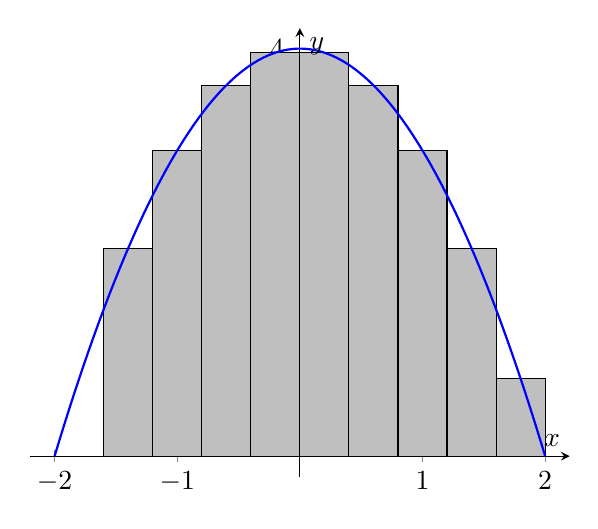
\begin{tikzpicture}
  \begin{axis}[
      xlabel=$x$,
      ylabel=$y$,
      domain=-2:2,
      samples=100,
      axis lines=middle,
      xtick={-2,-1,0,1,2},
      ytick={0,1,2,3,4},
      xmin=-2.2,
      xmax=2.2,
      ymin=-0.2,
      ymax=4.2,
  ]
  \pgfplotsinvokeforeach{-1.6,-1.2,...,1.6}{
      \draw[fill=gray!50] (#1,0) rectangle (#1+0.4,{-(#1+0.2)^2+4});
  }
  \addplot[blue, thick] {-x^2+4};
  \end{axis}
\end{tikzpicture}
\end{center}

\end{multicols}


\section{Indefinite Integrals (Calc Book Part 9)}

% Part A
\[\int 35 x^6 dx =\quad \frac{35^7}{7}+c = 5^7+c\]
\[\int \frac{63}{t^8}dt = \int 63\cdot t^{-8} dx = \frac{63t^{-8+1}}{-8+1}+c= \frac{63t^{-7}}{-7}+c = -\frac{9}{t^7}+c\]
\[\int 15x^{2/3}dx=\quad \frac{15x^{5/3}}{5/3}+c = 9x^{5/3}+c\]
\[\int 48u^{-5}du= \frac{48u^{-4}}{-4}+c =\quad -12^{-4u}+c\]

% Part B
\[\int t dt =\quad \frac{t^2}{2}+c\]
\[\int \frac{dx}{\sqrt{x}}=\quad \int x^{-1/2}dx =\quad \frac{x^{1/2}}{1/2}+c=\quad 2\sqrt{x}+c\]
\[\int 4 du =\quad 4u+c\]
\[\int \frac{8dx}{x^{1/3}} =\quad \int 8x^{-1/3}dx =\quad \frac{8x^{-1/3+1}}{-\frac{1}{3}+1}+c = \frac{8x^{2/3}}{2/3}+c = 12x^{2/3}+c \]

% Part C
\[\int (x^2-3x+4)dx =\quad \frac{x^3}{3}-1,5x^2+4x+c\]
\[\int \left(\frac{1}{u^2}-\frac{4}{u}\right)dx = \dots = -\frac{1}{u}-4\ln\footnote{Recall that a power of $b=-1$ is a special case : $\int \frac{du}{u}=\int u^{-1}du=\ln u+c$} u+c \]
\[\int (10x^{3/2}+6x^{1/2})\ dx =\quad \frac{10x^{5/2}}{5/2}+\frac{6x^{3/2}}{3/2}+c = 4x^{5/2}+4x^{3/2}+c\]
\[\int \left(\sqrt{t}+\frac{1}{\sqrt{t}}\right)\ dt =\quad \frac{t^{3/2}}{3/2}+\frac{t^{-3/2}}{1/2}+c= \frac{2t^{3/2}}{3}+2t^{1/2}+c \]

\clearpage

\section{Und hier eine ``ganze'' Integralerklaerung}
\begin{multicols}{2}
  \subsection{Erst die einfachen Regeln}
  \[\int ax^b\ dx= \frac{ax^{b+1}}{b+1}+c, (\text{wenn b $\ne$ -1})\]
  \[\int x^{-1}\ dx = \int \frac{dx}{x} = \ln x + c\]
  \[\int \sin \theta\ d\theta = -\cos \theta + c\]
  \[\int \cos \theta\ d\theta = \sin \theta + c\]
  \[\int e^{ax}\ dx= \frac{e^{ax}}{a}+c\]
  \[\int b^x\ dx = \frac{b^x}{\ln b} + c\]

\ex{ \[\int 12x^3\ dx \]
      Hier f\"angt man an es mit der ersten regel zu integrieren:
      \[ = \frac{12x^{3+1}}{3+1} = \frac{12x^{4}}{4} \]
      Das k\"urzt man dann auf $3x^4 (+c)$. }

\ex{
  \[ \int\left(\frac{1}{u^2}-\frac{4}{u}\right)\ du \]
  \[ =-\frac{1}{u} -4 \to -\ln u-4+c\]
}

\ex{
  \[ \int\left(\sqrt{t}+\frac{1}{\sqrt{t}\ dt}\right) \]
  \[ = \frac{t^{3/2}}{3/2}+\frac{\sqrt{t}}{2}+c \]
}

Definierte Integrale: diese sind auf der x-Achse definiert, um ihre Fl\"ache zu finden
\end{multicols}
